\documentclass[aspectratio=169]{beamer}
\usetheme{Madrid}
\usepackage[utf8]{inputenc}
\usepackage[T1]{fontenc}
\usepackage{tikz}
\usepackage{amssymb}
\usepackage{graphicx}
\setbeamertemplate{navigation symbols}{}
\setbeamercolor{title}{fg=white,bg=magenta!70!red}
\setbeamercolor{frametitle}{fg=white,bg=magenta!70!red}
\setbeamercolor{block title}{bg=magenta!70!red!20,fg=black}
\setbeamercolor{block body}{bg=magenta!70!red!8,fg=black}
\setbeamercolor{item}{fg=magenta!70!red}
\setbeamercolor{itemize item}{fg=magenta!70!red}
\setbeamertemplate{itemize item}[triangle]

\title{Foundations 1 — What Is a Computer?}
\subtitle{CPU, RAM, storage, input/output — the real physical parts}
\author{ByteForge --- Grade 9 --- The Deep Diver}
\date{}

\begin{document}

\begin{frame}
    \titlepage
\end{frame}

\begin{frame}{Today's Missions}
    \Large
    \begin{itemize}
        \item Learn: What Is a Computer?
        \item RAM or Storage?
        \item Input, Process, or Output?
        \item Storage Unit Conversion
        \item Pick the Right Storage
    \end{itemize}
\end{frame}

\begin{frame}{A computer is really just 4 jobs}
    \large
    \begin{itemize}
        \item INPUT --- getting information IN (keyboard, mouse, a sensor)
        \item PROCESS --- the CPU actually doing the thinking/calculating
        \item OUTPUT --- showing a result (screen, speaker, printer)
        \item STORAGE --- keeping data around, even with the power off
    \end{itemize}
\end{frame}


\begin{frame}{RAM vs. Storage --- the single most confused pair}
    \large
    \begin{itemize}
        \item RAM = short-term memory --- FAST, but wiped the instant power is lost
        \item Storage (a hard drive/SSD) = long-term memory --- slower, but survives being switched off
        \item Closing your laptop lid without saving = the essay was only ever in RAM
    \end{itemize}
\end{frame}


\begin{frame}{The CPU is the "brain", but it is very literal}
    \large
    \begin{itemize}
        \item It only ever does exactly what its instructions say --- nothing more
        \item Billions of tiny operations every second, but each one is dead simple
        \item "Smart" behaviour is really just A LOT of simple steps, very fast
    \end{itemize}
\end{frame}


\begin{frame}{Storage units --- each one is 1024x the last}
    \large
    \begin{itemize}
        \item 8 bits = 1 byte --- enough to store one single character
        \item 1024 bytes = 1 KB, 1024 KB = 1 MB, 1024 MB = 1 GB, 1024 GB = 1 TB
        \item A text message: a few hundred bytes. A phone photo: a few MB. A whole phone: measured in GB
    \end{itemize}
\end{frame}


\begin{frame}{Not all storage devices work the same way}
    \large
    \begin{itemize}
        \item HDD --- a spinning magnetic disk, cheap and large, but slower with moving parts that wear out
        \item SSD --- NO moving parts, genuinely faster and more reliable, usually costs more per GB
        \item Cloud --- not really a different type at all, just storage in someone else's data centre, reached over the internet
    \end{itemize}
\end{frame}

\begin{frame}{Real-World Examples}
    \large
    \begin{itemize}
        \item Every phone, games console, and smart fridge is doing the exact same 4 jobs --- input, process, output, storage --- just in a different shaped box.
        \item A Minecraft server genuinely runs on this: player commands are INPUT, world logic is PROCESSED, what you see is OUTPUT, and the saved world is STORAGE.
    \end{itemize}
\end{frame}


\begin{frame}{Image}
    \begin{center}
    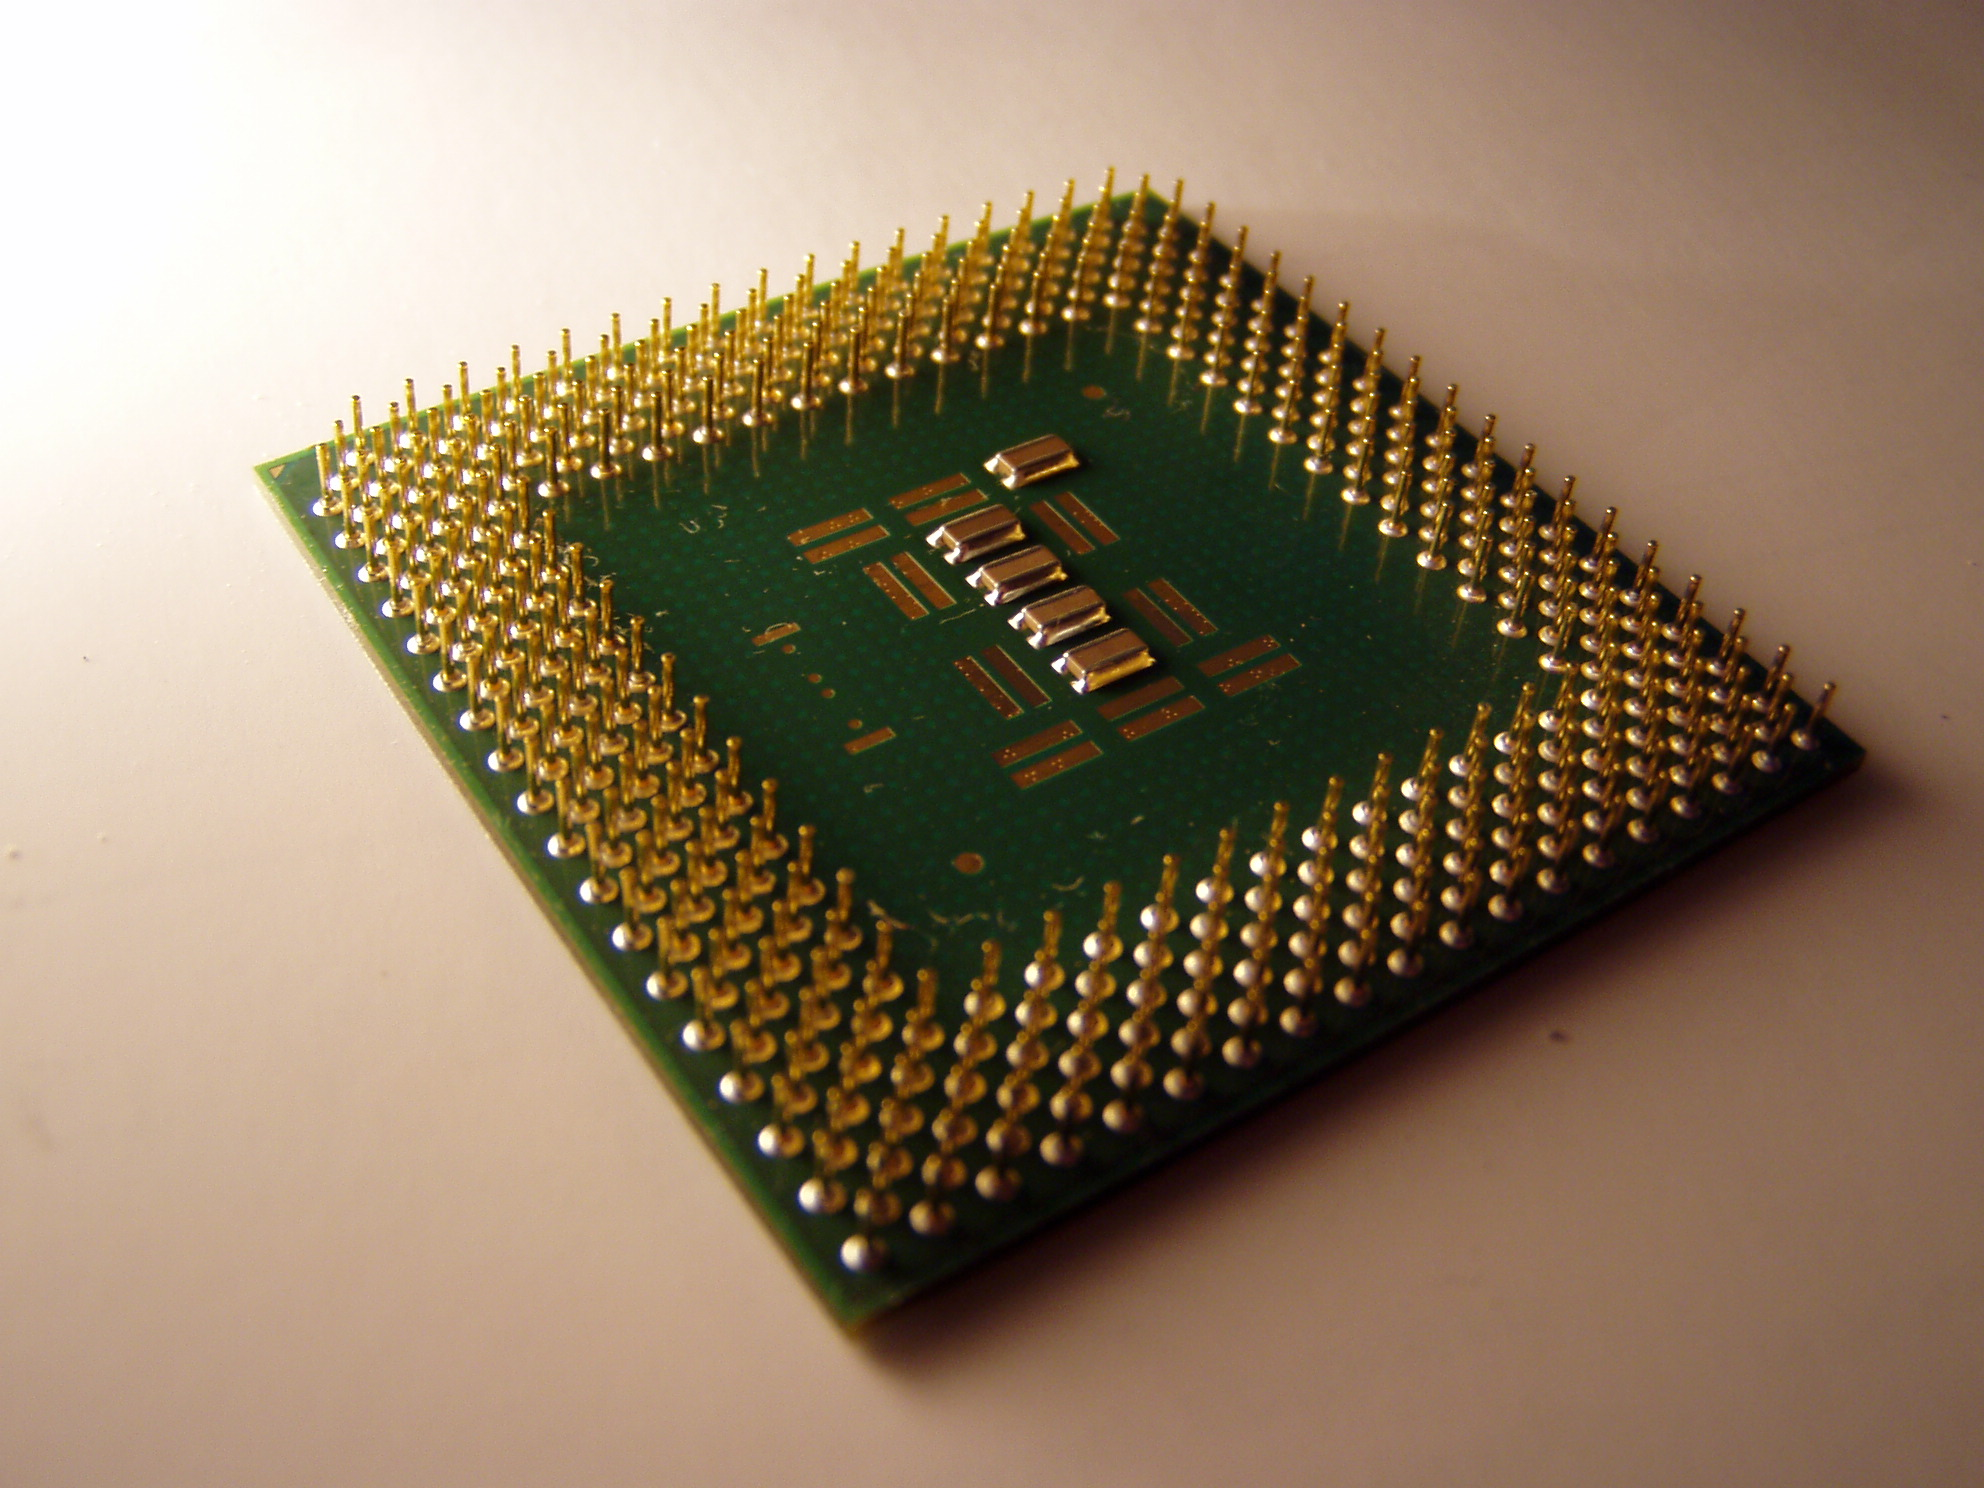
\includegraphics[width=0.5\textwidth]{images/cpu.jpg}

    \large A real CPU --- hundreds of gold pins, each one carrying a real electrical signal in or out.

    \small CPU photo --- Poooow, public domain, via Wikimedia Commons
    \end{center}
\end{frame}


\begin{frame}{Image}
    \begin{center}
    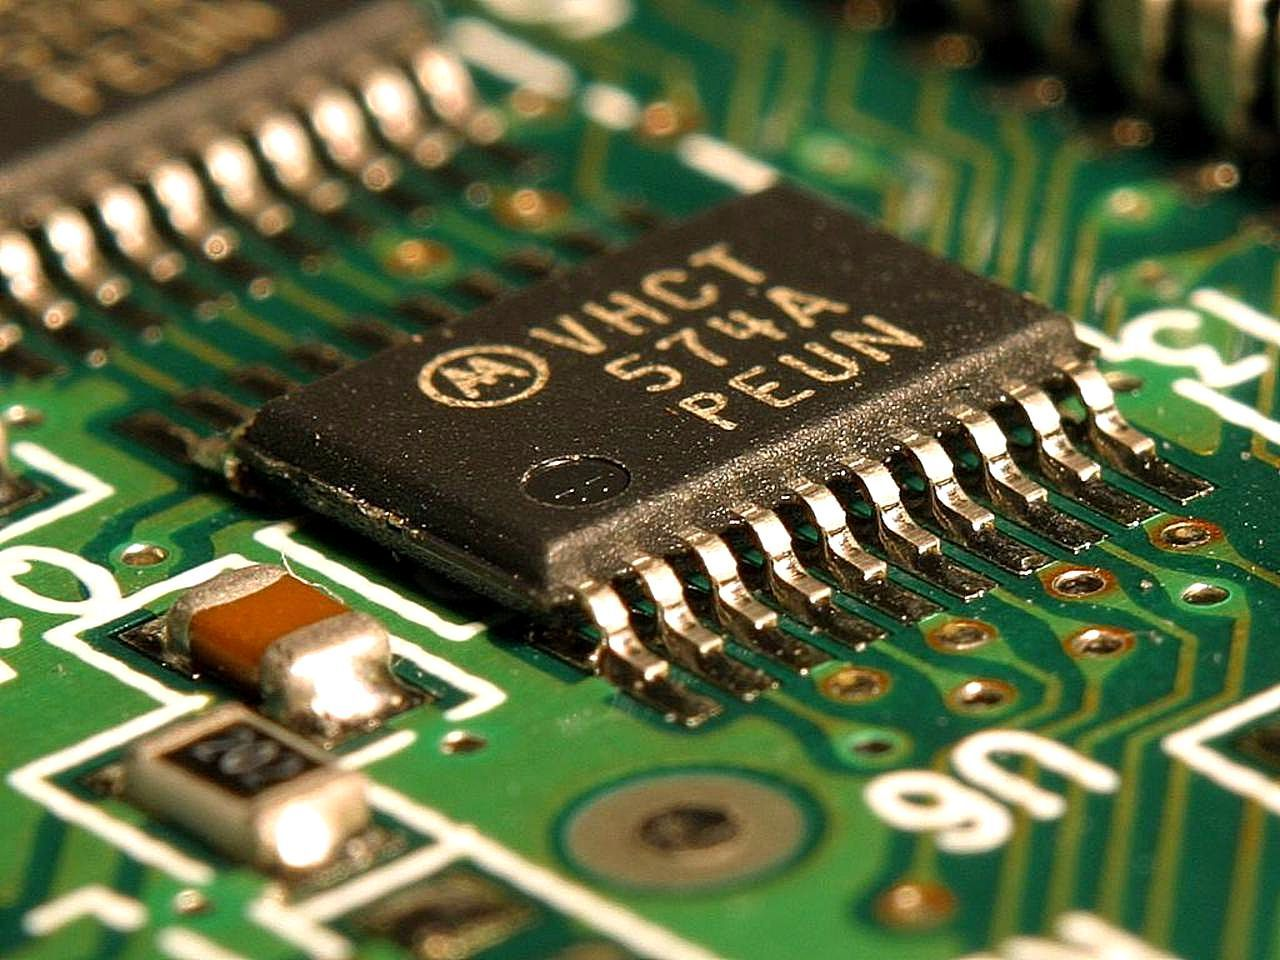
\includegraphics[width=0.5\textwidth]{images/circuit.jpg}

    \large Real circuitry --- this is genuinely what "processing" looks like up close.

    \small Circuit board, Jon Sullivan, public domain, via Wikimedia Commons
    \end{center}
\end{frame}

\begin{frame}{Let Them Discover (1/2)}
    \large
    Open Task Manager (or Activity Monitor) and find how much RAM is currently in use. Now find how much storage space is free. Why are these two totally different numbers?
\end{frame}


\begin{frame}{Let Them Discover (2/2)}
    \large
    List 3 things your phone does that are pure OUTPUT, and 3 that are pure INPUT. Is anything genuinely both at once (hint: a touchscreen)?
\end{frame}

\begin{frame}{Your Turn}
    \Large
    Open the mission map, find \textbf{Foundations 1 — What Is a Computer?}, and fly it for real ---
    everything you just saw, you now do yourself.
\end{frame}

\end{document}
